\documentclass{article}
\usepackage[utf8]{inputenc}
\usepackage{enumitem}
\usepackage{ulem}
\usepackage{mathrsfs}
\usepackage{amsmath}
\usepackage{float}
\usepackage{hyperref}
\usepackage{xcolor}
\usepackage{listings}
\usepackage{color}
\usepackage[utf8]{inputenc}
\usepackage{CJK}
\usepackage{amsthm,amsmath,amssymb}
\usepackage{hyperref}
\usepackage{relsize}
\usepackage{graphicx}
\usepackage{mathtools}
\usepackage{tikz}

\newtheorem{problem}{Problem}

\newcommand{\N}{\mathcal N}
\newcommand{\Y}{\mathbf Y}
\newcommand{\real}{\mathbb{R}}
\newcommand{\X}{\mathbf X}
\newcommand{\Z}{\mathbf Z}

\newcommand*{\tran}{^{\mkern-1.5mu\mathsf{T}}}
\newcommand*{\hermitian}{^{\mkern-1.5mu\mathsf{H}}}

\newcommand{\Tau}{\mathrm{T}}

\DeclareMathOperator{\Tr}{Tr}

\def\Epsilon{E}
\def\Eta{H}

\def\veczero{{\mathbf 0}}
\def\vec1{{\mathbf 1}}
\def\matzero{{\mathbf 0}}

\def\veca{{\mathbf a}}
\def\vecb{{\mathbf b}}
\def\vecc{{\mathbf c}}
\def\vecd{{\mathbf d}}
\def\vece{{\mathbf e}}
\def\vecf{{\mathbf f}}
\def\vecg{{\mathbf g}}
\def\vech{{\mathbf h}}
\def\veck{{\mathbf k}}
\def\vecm{{\mathbf m}}
\def\vecn{{\mathbf n}}
\def\vecp{{\mathbf p}}
\def\vecq{{\mathbf q}}
\def\vecr{{\mathbf r}}
\def\vect{{\mathbf t}}
\def\vecu{{\mathbf u}}
\def\vecv{{\mathbf v}}
\def\vecw{{\mathbf w}}
\def\vecx{{\mathbf x}}
\def\vecy{{\mathbf y}}
\def\vecz{{\mathbf z}}

\def\vecalpha{{\mathbf \alpha}}
\def\vecbeta{{\mathbf \beta}}
\def\vecepsilon{{\boldsymbol \epsilon}}
\def\veclambda{{\mathbf \lambda}}
\def\vecvarepsilon{{\boldsymbol \varepsilon}}
\def\vecgamma{{\boldsymbol \gamma}}
\def\vecmu{{\boldsymbol \mu}}
\def\vecnu{{\boldsymbol \nu}}
\def\vecomega{{\boldsymbol \omega}}
\def\vecphi{{\boldsymbol \phi}}
\def\vecpsi{{\boldsymbol \psi}}
\def\vecsigma{{\mathbf \sigma}}
\def\vecvarsigma{{\mathbf \varsigma}}
\def\vectau{{\boldsymbol \tau}}
\def\vecupsilon{{\boldsymbol \upsilon}}
\def\vecvarphi{{\boldsymbol \varphi}}
\def\vecxi{{\boldsymbol \xi}}
\def\veczeta{{\boldsymbol \zeta}}


\def\vecX{{\mathbf X}}
\def\vecY{{\mathbf Y}}
\def\vecZ{{\mathbf Z}}

\def\vecEpsilon{{\mathbf \Epsilon}}
\def\vecEta{{\mathbf \Eta}}


\def\matA{{\mathbf A}}
\def\matB{{\mathbf B}}
\def\matC{{\mathbf C}}
\def\matD{{\mathbf D}}
\def\matE{{\mathbf E}}
\def\matF{{\mathbf F}}
\def\matH{{\mathbf H}}
\def\matI{{\mathbf I}}
\def\matK{{\mathbf K}}
\def\matL{{\mathbf L}}
\def\matO{{\mathbf O}}
\def\matOmega{{\mathbf \Omega}}
\def\matN{{\mathbf N}}
\def\matP{{\mathbf P}}
\def\matS{{\mathbf S}}
\def\matU{{\mathbf U}}
\def\matV{{\mathbf V}}
\def\matW{{\mathbf W}}
\def\matX{{\mathbf X}}
\def\matZ{{\mathbf Z}}
\def\matGamma{{\mathbf{\mathrm{\Gamma}}}}
\def\matLambda{{\mathbf{\mathrm{\Lambda}}}}
\def\matOmega{{\mathbf{\mathrm{\Omega}}}}
\def\matPhi{{\mathbf \Phi}}
\def\matPsi{{\mathbf \Psi}}
\def\matRho{{\mathbf{\mathrm{P}}}}
\def\matSigma{{\mathbf{\mathrm{\Sigma}}}}
\def\matUpsilon{{\mathbf{\mathrm{\Upsilon}}}}
\def\matXi{{\mathbf{\mathrm{\Xi}}}}

\def\matzero{{\mathbf 0}}


\def\complex{{\mathbb {C}}}
\def\real{{\mathbb {R}}}
\def\extreal{\overline{\mathbb {R}}}
\def\rational{{\mathbb {Q}}}
\def\pnint{{\mathbb {Z}}}
\def\nnint{{\mathbb{N}_0}}
\def\pint{{\mathbb {N}}}
\def\extint{\overline{\mathbb {Z}}}

\def\defas{:=}
\def\as{\overset{\mbox{a.s.}}{=}}
\def\ind{1}
\def\normal{\calN}
\def\expect{\mathbb{E}}
\def\variance{\mbox{Var}}
\def\covariance{\mbox{Cov}}
\def\prob{\mathbb{P}}
\def\risk{\calR}
\def\Uniform{{\cal{U}}}
\def\Trace{\mbox{Tr}}
\def\sign{\mbox{sign}}
\def\evaloss{\star}
\def\margin{\varrho}
\def\Log{{Log}}

\def\converged{\xrightarrow[]{D}}
\def\convergep{\xrightarrow[]{P}}
\def\convergeas{\xrightarrow[]{a.s.}}

\def\Borel{{\frakB}}

\def\Re{\mbox{Re}}
\def\Im{\mbox{Im}}

\def\interior{\mathrm{o}}

\def\calA{{\cal A}}
\def\calB{{\cal B}}
\def\calC{{\cal C}}
\def\calD{{\cal D}}
\def\calE{{\cal E}}
\def\calF{{\cal F}}
\def\calG{{\cal G}}
\def\calH{{\cal H}}
\def\calK{{\cal K}}
\def\calL{{\cal L}}
\def\calM{{\cal M}}
\def\calN{{\cal N}}
\def\calP{{\cal P}}
\def\calR{{\cal R}}
\def\calS{{\cal S}}
\def\calT{{\cal T}}
\def\calV{{\cal V}}
\def\calX{{\cal X}}
\def\calY{{\cal Y}}
\def\calZ{{\cal Z}}

\def\scrA{\mathscr{A}}
\def\scrB{\mathscr{B}}
\def\scrC{\mathscr{C}}
\def\scrD{\mathscr{D}}
\def\scrE{\mathscr{E}}
\def\scrF{\mathscr{F}}
\def\scrG{\mathscr{G}}
\def\scrI{\mathscr{I}}
\def\scrJ{\mathscr{J}}
\def\scrK{\mathscr{K}}
\def\scrL{\mathscr{L}}
\def\scrM{\mathscr{M}}
\def\scrN{\mathscr{N}}
\def\scrP{\mathscr{P}}
\def\scrQ{\mathscr{Q}}
\def\scrR{\mathscr{R}}
\def\scrS{\mathscr{S}}
\def\scrU{\mathscr{U}}
\def\scrV{\mathscr{V}}
\def\scrX{\mathscr{X}}


\def\pzch{\mathpzc{h}}
\def\pzcy{\mathpzc{y}}

\def\frakA{\mathfrak{A}}
\def\frakB{\mathfrak{B}}
\def\frakG{\mathfrak{G}}
\def\frakM{\mathfrak{M}}

\def\continuous{{\cal C}}


\addtolength{\oddsidemargin}{-.875in}
\addtolength{\evensidemargin}{-.875in}
\addtolength{\textwidth}{1.75in}
\addtolength{\topmargin}{-.875in}
\addtolength{\textheight}{1.75in}


\title{HW3 Handwritten Assignment}
\author{Lecturor: Pei-Yuan Wu\\
TAs: {Yuan-Chia Chang(Problem 1, 2), Chun-Lin Huang(Problem 3, 4, 5)}}
\date{October 2023, Second Edition}
\begin{document}

\maketitle

\section*{Problem 1 (LSTM Cell)(0.5\%)}
In this exercise, we will simulate the forward pass of a simple LSTM cell. Figure.1 shows a single LSTM cell, where $z$ is the cell input, $z_i, z_f, z_o$ are the control inputs of the gates, $c$ is the cell memory, and $f, g, h$ are activation functions. Given an input $x$, the cell input and the control inputs can be calculated by the following equations :
\begin{itemize}
    \item $z = w \cdot x + b$
    \item $z^i = w_i \cdot x + b_i$
    \item $z^f = w_f \cdot x + b_f$
    \item $z^o = w_o \cdot x + b_o$
\end{itemize}
where $w, w_i, w_f, w_o$ are weights and $b, b_i, b_f, b_o$ are biases. The final output can be calculated by
$$y = f(z^o)\ h(c')$$
where the value stored in cell memory is updated by
$$c'=f(z^i)g(z)+cf(z^f)$$
Note that $f(z) = \frac{1}{1+e^{-z}}\quad , g(z) = z,\quad h(z) = z$

Given an input sequence $x^t\ ( t = 1, 2, 3, 4 )$, please derive the output sequence $y_t$. The input sequence, the weights, and the activation functions are provided below. 
\begin{equation*}
\begin{array}{ll}
w=[0,0,1,0] & , b=0 \\
w_i=[50,50,0,0] & , b_i=-5 \\
w_f=[-50,-50,0,0], & , b_f=120 \\
w_o=[0,0,200,0] & , b_0=-30\\
x^1 = [0,0,1,3] &,x^2=[0,1,-1,2]\\
x^3=[2,1,3,4]&, x^4=[0,1,0,0]
\end{array}
\end{equation*}
The initial value in cell memory is 0. \textbf{Please note that your calculation process is required to receive full credit.}
\newpage
\begin{figure}[h]
    \centering
    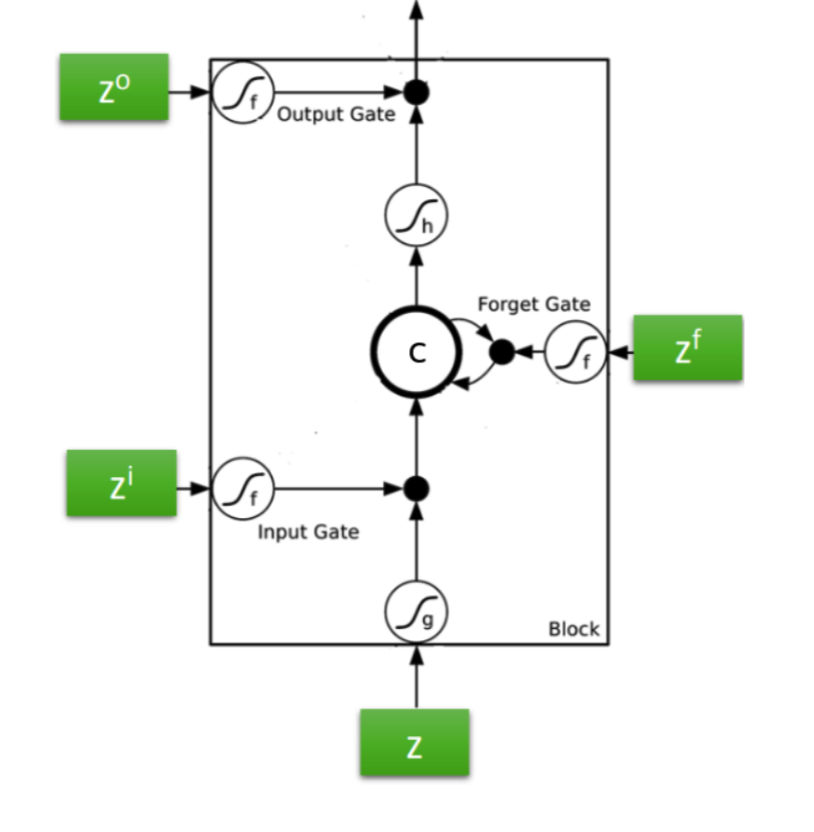
\includegraphics[width=0.8\textwidth]{LSTM.png}
    \caption{Problem 1 LSTM model}
\end{figure}

\section*{Problem 2 (Laplacian Eigenmaps)(1.5\%)}
Consider an undirected connected graph $G$, which is shown below. We want to utilize Laplacian Eigenmaps method to reduce these 10 points to 3-dimensional space. Here, undirected graph means that edges in the graph  do not have a direction, and connected graph means that there is a path from any node to any other node in the graph.
\begin{figure}[ht!]
        \centering
    \begin{tikzpicture}[main/.style = {draw, circle}]
    \node[main] (1) {$x_1$}; 
    \node[main] (2) [below right of=1] {$x_2$}; 
    \node[main] (3) [below left of=1] {$x_3$}; 
    \node[main] (4) [above right of=1] {$x_4$}; 
    \node[main] (9) [below left of=3] {$x_9$}; 
    \node[main] (10) [below right of=3] {$x_{10}$}; 
    \node[main] (8) [above of=4] {$x_8$}; 
    \node[main] (7) [below right of=10] {$x_7$}; 
    \node[main] (5) [right of=7] {$x_5$}; 
    \node[main] (6) [right of=5] {$x_6$};
    \draw (1) -- (2); 
    \draw (1) -- (3); 
    \draw (1) -- (4);
    \draw (2) -- (4); 
    \draw (2) to [out=45,in=45,looseness=1.5]  (8);
    \draw (3) to [out=135,in=135,looseness=1.5]  (8);
    \draw (5) -- (6); 
    \draw (5) -- (7); 
    \draw (7) -- (10); 
    \draw (8) to [out=90,in=180,looseness=3]  (9);
    \draw (9) -- (10); 
    \end{tikzpicture}
        \caption{Problem 2 undirected connected graph $G$}
    \end{figure}


\begin{enumerate}
    \item Write down the adjacency matrix $\boldsymbol{W}$
    \item Write down the diagonal matrix $\boldsymbol{D}=diag(d_1,...,d_{10})$, where $d_i=\sum_{j=1}^{10} \frac{\boldsymbol{W_{ij}}+\boldsymbol{W_{ji}}}{2}$ and the Laplacian $\boldsymbol{L}=\boldsymbol{D}-\boldsymbol{W}$.
    \item By HW2 Problem 3, Neighbor Embedding Slide p.7-p.10 and programming tools(MATLAB, Python...), solve the optimization problem \\
minimize  $\quad Trace(\boldsymbol{\Psi}^T \boldsymbol{L} \boldsymbol{\Psi})$ \\ 
subject to $\quad \boldsymbol{\Psi}^T \boldsymbol{D} \boldsymbol{\Psi} = \boldsymbol{I}_3$ \\
variables $\quad \boldsymbol{\Psi} \in \mathbb{R}^{10 \times 3}$ \\
Also, please plot the reduced points $\boldsymbol{z_1},...,\boldsymbol{z_{10}}$ in 3-D scatter plot.
\item You may find that the minimal eigenvalue of $\boldsymbol{L}$ is 0, and the corresponding eigenvector is 
\begin{align}
    \begin{bmatrix}
       c \\
       c \\
       \vdots \\
       c
     \end{bmatrix}
  \end{align}
  where $c$ is a constant. Since all the points fall into a plane, the span of these points is $\mathbb{R}^2$. In order to construct $\boldsymbol{z_1},...,\boldsymbol{z_{10}}$ such that span\{$\boldsymbol{z_1},...,\boldsymbol{z_{10}}\}=\mathbb{R}^3$, we need choose the second, third, fourth smallest eigenvalue and the corresponding eigenvectors. Please plot the reduced points by the updated $\boldsymbol{z_1},...,\boldsymbol{z_{10}}$ in 3-D scatter plot and verify that whether 
$\quad Trace(\boldsymbol{\Psi}^T \boldsymbol{L} \boldsymbol{\Psi})=1.098$ \ and $\quad \boldsymbol{\Psi}^T \boldsymbol{D} \boldsymbol{\Psi} = \boldsymbol{I}_3$.

\item Show that for no matter the graph is, there is an eigenvector of $\boldsymbol{L}$ 
\begin{align}
    \begin{bmatrix}
       c \\
       c \\
       \vdots \\
       c
     \end{bmatrix}
  \end{align}
  where $c$ is a constant, and the corresponding eigenvalue is 0.

\item By Neighbor Embedding Slide p.9, please show that \\
$ \forall \boldsymbol{f} =$
$\begin{bmatrix}
   f_1 \\
   f_2 \\
   \vdots \\
   f_N
\end{bmatrix}$
$\in \mathbb{R}^N, \boldsymbol{f}^T \boldsymbol{L} \boldsymbol{f}=\frac{1}{2}\sum\limits_{1 \leq i,j \leq N} w_{ij}(f_i-f_j)^2$.
\item Show that if $\boldsymbol{f}$ is an eigenvector of $\boldsymbol{L}$ which corresponds to eigenvalue 0, then $\boldsymbol{f}^T \boldsymbol{L} \boldsymbol{f}=0$.
\item Show that if the graph is connected, the second smallest eigenvalue 
 of $\boldsymbol{L}$ will be nonzero.

\end{enumerate}



\section*{Problem 3 (Multiclass AdaBoost)(1.5\%)}
Let $\mathcal{X}$ be the input space, $\mathscr F$ be a collection of multiclass classifiers that map from $\mathcal{X}$ to $[1, K]$, where $K$ denotes the number of classes.  Let $\{(x_i,{\hat y}_i)\}_{i=1}^m$ be the training data set, where $x_i \in \mathcal{X}$ and ${\hat y}_i \in [1,K]$.  Given $T \in \mathbb{N}$, suppose we want to find functions 
\begin{equation*}
g_{T+1}^k(x) = \sum_{t=1}^T \alpha_t f_t^k(x), ~~ k \in [ 1,K ]
\end{equation*}
where $f_t \in \mathscr F$ and $\alpha_t \in \mathbb{R}$ for all $t \in [1, T]$. Here for $f \in \mathscr F$, we denote $f^k(x) = \mathbf{1}\{f(x) = k\}$, where $\mathbf{1}(\cdot)$ is an indicator function, as the $k$'th element in the one-hot representation of $f(x) \in [ 1,K ]$. The aggregated classifier $h: \mathcal{X} \rightarrow [ 1,K ]$ is defined as
\begin{equation*}
x \mapsto \underset{1 \leq k \leq K}{\mbox{argmax}} ~ g_{T+1}^k(x)
\end{equation*}

Please apply gradient boosting to show how the functions $f_t$ and coefficients $\alpha_t$ are computed with an aim to minimize the following loss function
\begin{equation*}
L((g_{T+1}^1, \cdots, g_{T+1}^K) = \sum_{i=1}^m \exp\left(\frac{1}{K-1}\sum_{k \neq {\hat y}_i} g_{T+1}^{k}(x_i) - g_{T+1}^{{\hat y}_i}(x_i) \right)
\end{equation*}

\section*{Problem 4 (Backpropagation through time via Simple RNN)(1\%)}
Backpropagation through time is a critical concept to know as we train a recurrent network. Here, we set a toy case of prediction problem. 
\begin{figure}[h]
    \centering
    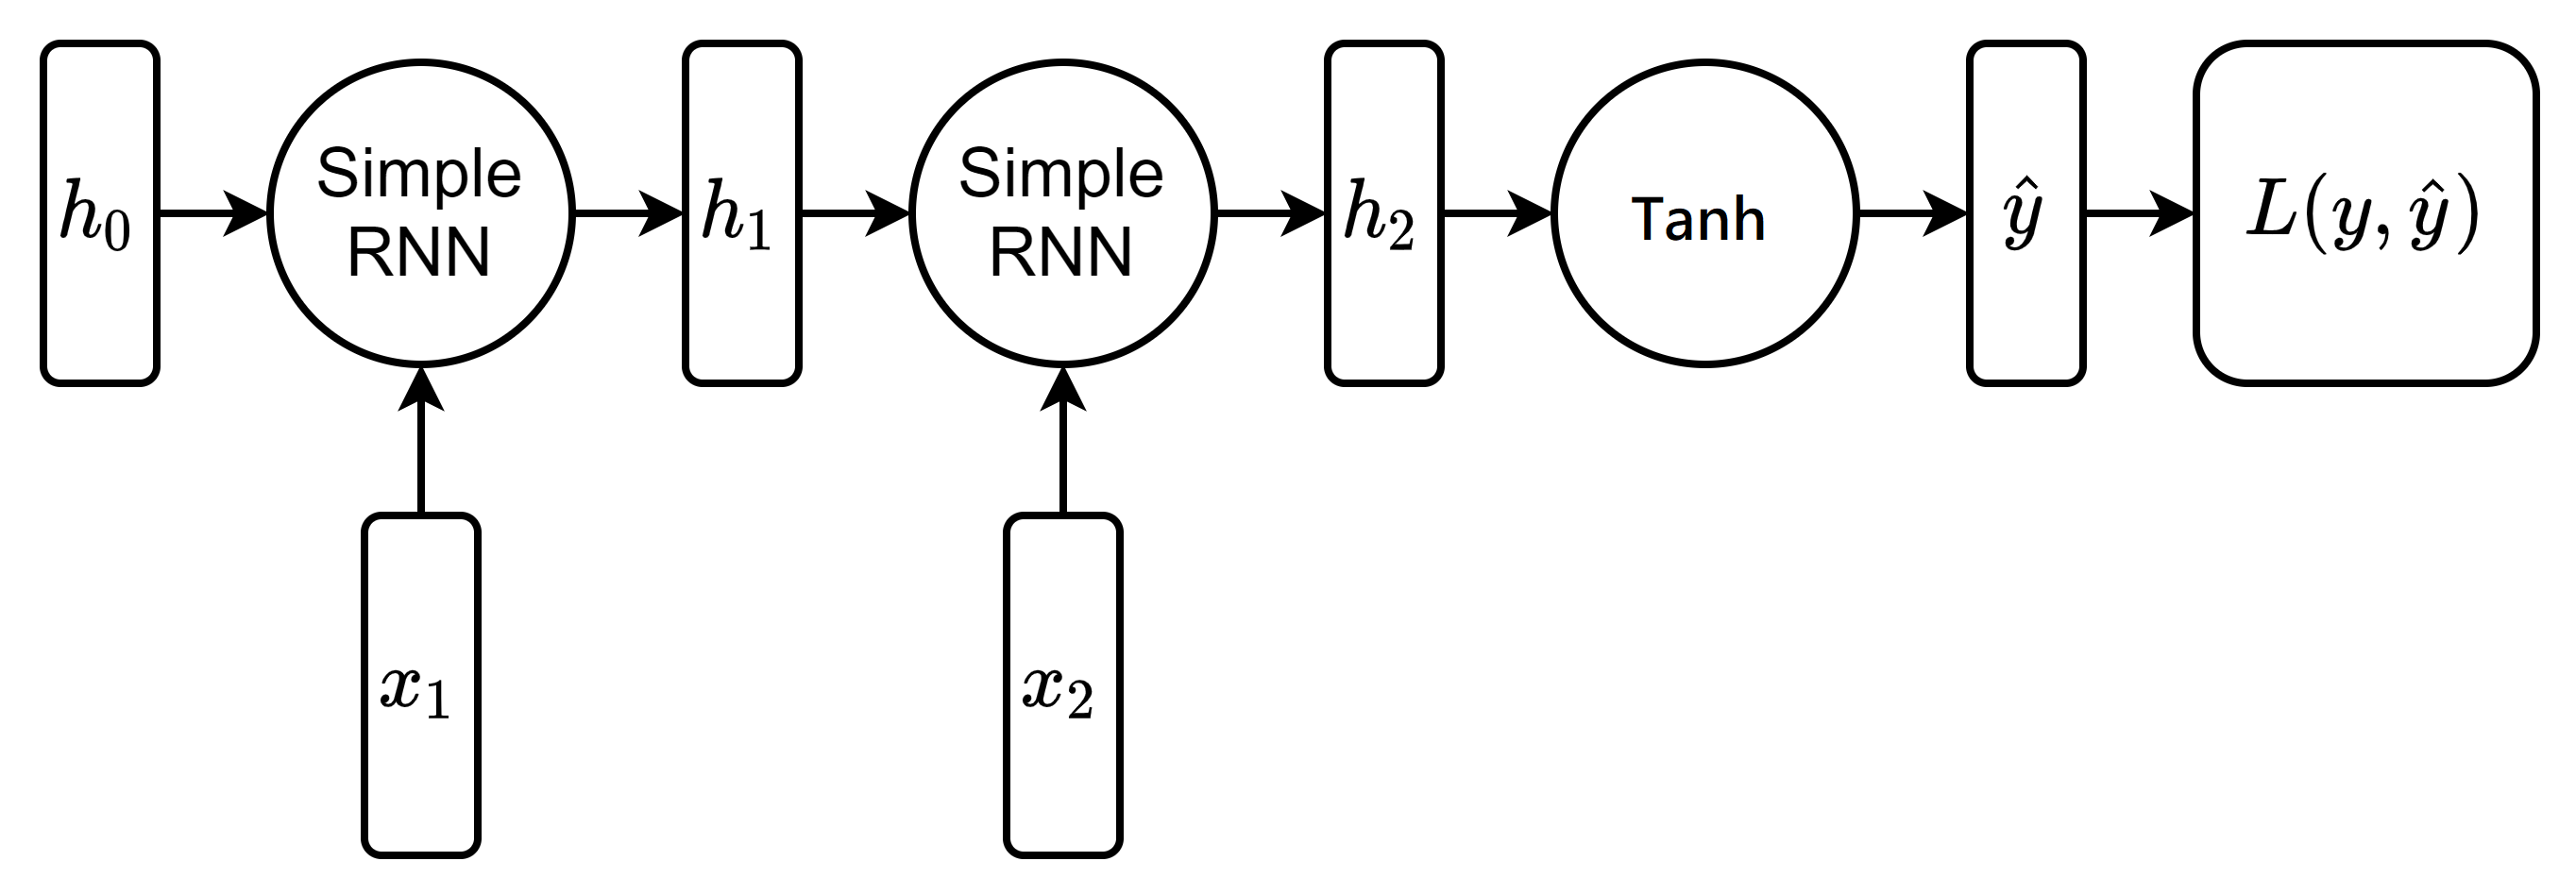
\includegraphics[width=0.8\textwidth]{RNN.png}
\end{figure}
The Simple RNN module has two kinds of weights, $w_x$ and $w_h$, such that $h_t = \text{tanh}(w_xx_t + w_hh_{t-1})$, where $t$ represents the index of steps. The module has the weight $w_o$ such that $\hat{y} = \sigma(w_o h_2)$, where $\sigma(w_oh_2) = \frac{1}{1+\text{exp}(-w_o h_2)}$. The initial state $h_0$ is set to be $0$. The sequential input only contains $\{x_1, x_2\}$; the label is $y$; the loss function is MSE. Please derive $\frac{\partial L(y, \hat{y})}{\partial w_o}$, $\frac{\partial L(y, \hat{y})}{\partial w_h}$, $\frac{\partial L(y, \hat{y})}{\partial w_x}$ in terms of $x_1$, $x_2$, $h_0$, $h_1$, $h_2$, $w_x$, $w_o$, and $w_h$.



\section*{Problem 5 (Loss function of Decision tree) (1.5\%)}
It is known that decision tree is still a powerful classification model now a days. There are two different loss functions when it comes to entropy counting, which are Shannon information gain and Gini index. Following are their definition:
\[
\text{Gini index} = \frac{N_{left}}{N}\left(1-\sum_{i=1}^c \left(p_{left}^i\right)^2\right) + \frac{N_{right}}{N}\left(1-\sum_{i=1}^c \left(p_{right}^i\right)^2\right)
\]
\[
\text{Shannon information gain} = \frac{N_{left}}{N}\left(-\sum_{i=1}^c p_{left}^i \log_2p_{left}^i\right) + \frac{N_{right}}{N}\left(-\sum_{i=1}^c p_{right}^i \log_2p_{right}^i\right)
\]
$p_i^j \coloneqq$ the proportion of class $j$ in the node $i$.\\
$N_i \coloneqq$ the number of cases in the node $i$.\\
Now we give a toy example. In this case $N_{left} = 8,p_{left}^1=\frac{5}{8},p_{left}^2=\frac{3}{8},N_{right}=12,p_{right}^1=\frac{5}{12},p_{right}^2=\frac{7}{12}$
\begin{figure}[h]
    \centering
    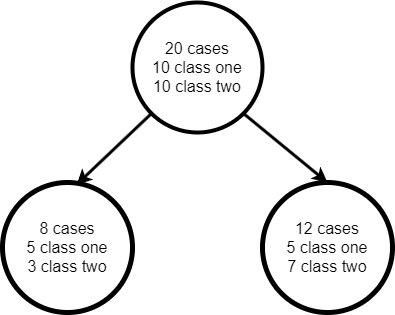
\includegraphics[width=0.4\textwidth]{ex_dt.png}
\end{figure}


In the following questions we consider classification of two cases. Please calculate the entropy of the following questions using two above-mentioned loss functions.
\begin{enumerate}[label=(\alph*)]
\item 
\begin{enumerate}[label=(\roman*)]
    \item A $50/50$ split with the first part containing $80 \%$ of positive examples and the second part containing $75 \%$ of positive examples.
    \item A $80/20$ split with the first part containing $0 \%$ of positive examples and the second part containing $90 \%$ of positive examples.
    \item A $90/10$ split with the first part containing $1 \%$ of positive examples and the second part containing $100 \%$ of positive examples.
\end{enumerate}
\item However, now suppose that our case is to detect the covid-19. Thus, we want our entropy function can have a higher loss on (iii) than (ii).Please decide a function that fulfill this criteria and write down the loss.
\end{enumerate}


 \section*{Version Description}
 \begin{enumerate}
     \item First Edition: Finish Problem 1 to 5
     \item Second Edition: Updated Problem 2(4) 2(5) 2(6) 2(7)'s typo
 \end{enumerate}
\end{document}
